\problemname{\problemyamlname}

\begin{wrapfigure}{r}{5.5cm}
    \centering
    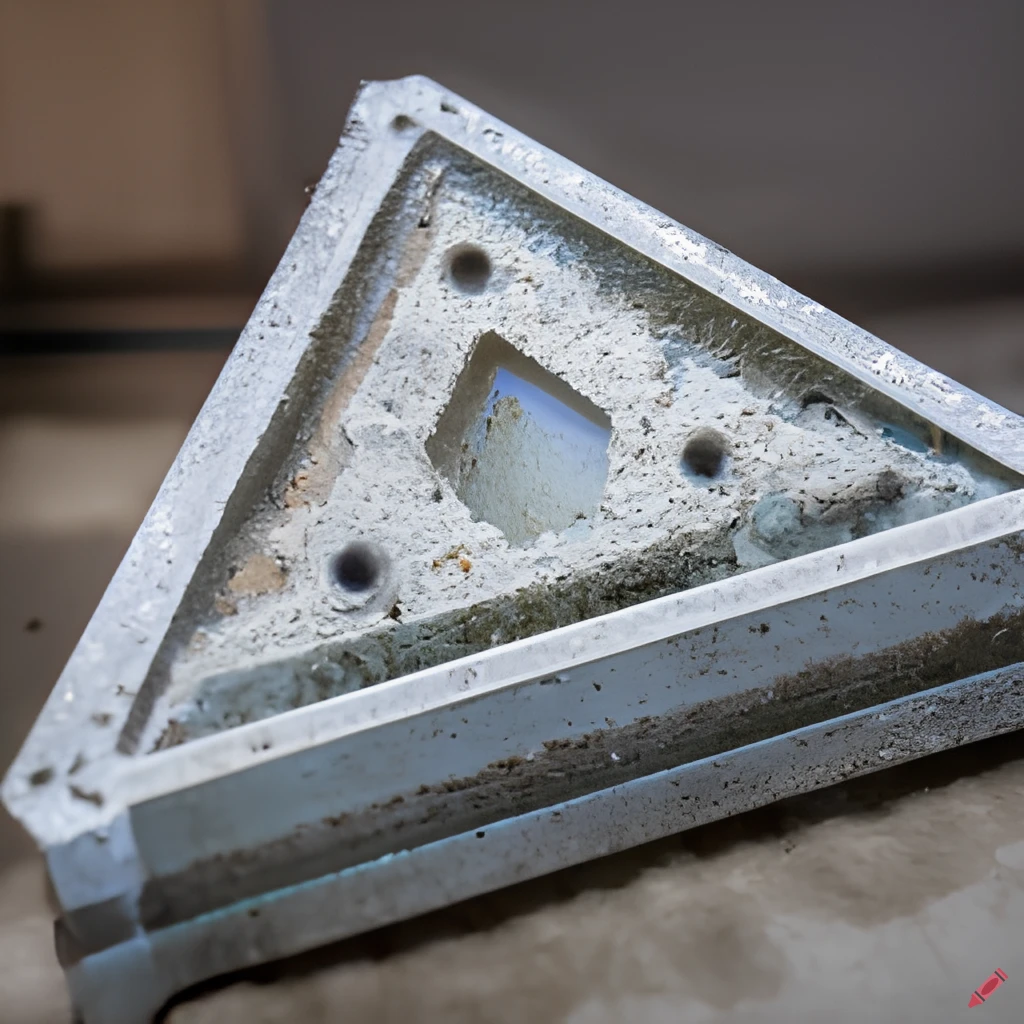
\includegraphics[width=5.5cm]{palindromium.jpg}
\end{wrapfigure}

A debate has started between the students of UMons and UCLouvain.
They can't decide on the best of the two universities, especially in the sciences.
They need your help to decide and advantage your university on the subject of a brand new metal called ``palindronium''.

Your mission is to optimize the production of palindronium in your university, production which is very costly at the moment.
To optimize it, the metal must be produced in a mold of the form of a right-angled triangle who's hypotenuse is a whole number and a palindrome.
Because of space constraints, you can only model a single mold, and it must fit in a square of size $n \times n$.
It must thus have a maximal area.

\begin{figure}[h]
\centering
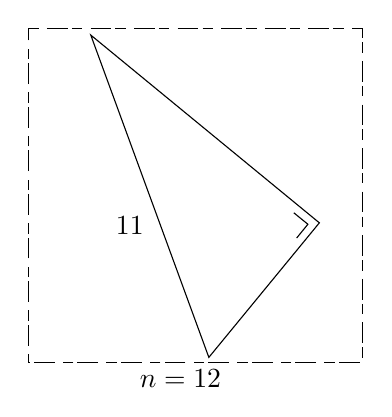
\begin{tikzpicture}[x=0.75pt,y=0.75pt,yscale=-1,xscale=1]
%uncomment if require: \path (0,300); %set diagram left start at 0, and has height of 300

%Shape: Rectangle [id:dp8053011662910811]
\draw  [dash pattern={on 3.75pt off 3pt on 7.5pt off 1.5pt}] (219.5,49.5) -- (380.75,49.5) -- (380.75,210.7) -- (219.5,210.7) -- cycle ;
%Shape: Right Triangle [id:dp47291251588999583]
\draw   (306.52,208.08) -- (249.63,52.79) -- (359.76,143.26) -- cycle ;
%Shape: Right Angle [id:dp6371826673456693]
\draw   (347.44,138.41) -- (354.24,143.94) -- (348.83,150.58) ;

% Text Node
\draw (260.5,139) node [anchor=north west][inner sep=0.75pt]   [align=left] {$\displaystyle 11$};
% Text Node
\draw (272,212.5) node [anchor=north west][inner sep=0.75pt]   [align=left] {$\displaystyle n=12$};
\end{tikzpicture}
\end{figure}

\begin{Input}
	An integer $n$ ($1 \le n \le 10^8$) which gives the length of the sides the square which must contain the triangular mold.
\end{Input}

\begin{Output}
	An integer which is the maximum area that you can get with a mold, with an absolute or relative error of maximum $10^{-6}$.
\end{Output}
